\documentclass[twoside]{book}

% Packages required by doxygen
\usepackage{fixltx2e}
\usepackage{calc}
\usepackage{doxygen}
\usepackage[export]{adjustbox} % also loads graphicx
\usepackage{graphicx}
\usepackage[utf8]{inputenc}
\usepackage{makeidx}
\usepackage{multicol}
\usepackage{multirow}
\PassOptionsToPackage{warn}{textcomp}
\usepackage{textcomp}
\usepackage[nointegrals]{wasysym}
\usepackage[table]{xcolor}

% Font selection
\usepackage[T1]{fontenc}
\usepackage[scaled=.90]{helvet}
\usepackage{courier}
\usepackage{amssymb}
\usepackage{sectsty}
\renewcommand{\familydefault}{\sfdefault}
\allsectionsfont{%
  \fontseries{bc}\selectfont%
  \color{darkgray}%
}
\renewcommand{\DoxyLabelFont}{%
  \fontseries{bc}\selectfont%
  \color{darkgray}%
}
\newcommand{\+}{\discretionary{\mbox{\scriptsize$\hookleftarrow$}}{}{}}

% Page & text layout
\usepackage{geometry}
\geometry{%
  a4paper,%
  top=2.5cm,%
  bottom=2.5cm,%
  left=2.5cm,%
  right=2.5cm%
}
\tolerance=750
\hfuzz=15pt
\hbadness=750
\setlength{\emergencystretch}{15pt}
\setlength{\parindent}{0cm}
\setlength{\parskip}{3ex plus 2ex minus 2ex}
\makeatletter
\renewcommand{\paragraph}{%
  \@startsection{paragraph}{4}{0ex}{-1.0ex}{1.0ex}{%
    \normalfont\normalsize\bfseries\SS@parafont%
  }%
}
\renewcommand{\subparagraph}{%
  \@startsection{subparagraph}{5}{0ex}{-1.0ex}{1.0ex}{%
    \normalfont\normalsize\bfseries\SS@subparafont%
  }%
}
\makeatother

% Headers & footers
\usepackage{fancyhdr}
\pagestyle{fancyplain}
\fancyhead[LE]{\fancyplain{}{\bfseries\thepage}}
\fancyhead[CE]{\fancyplain{}{}}
\fancyhead[RE]{\fancyplain{}{\bfseries\leftmark}}
\fancyhead[LO]{\fancyplain{}{\bfseries\rightmark}}
\fancyhead[CO]{\fancyplain{}{}}
\fancyhead[RO]{\fancyplain{}{\bfseries\thepage}}
\fancyfoot[LE]{\fancyplain{}{}}
\fancyfoot[CE]{\fancyplain{}{}}
\fancyfoot[RE]{\fancyplain{}{\bfseries\scriptsize Generated by Doxygen }}
\fancyfoot[LO]{\fancyplain{}{\bfseries\scriptsize Generated by Doxygen }}
\fancyfoot[CO]{\fancyplain{}{}}
\fancyfoot[RO]{\fancyplain{}{}}
\renewcommand{\footrulewidth}{0.4pt}
\renewcommand{\chaptermark}[1]{%
  \markboth{#1}{}%
}
\renewcommand{\sectionmark}[1]{%
  \markright{\thesection\ #1}%
}

% Indices & bibliography
\usepackage{natbib}
\usepackage[titles]{tocloft}
\setcounter{tocdepth}{3}
\setcounter{secnumdepth}{5}
\makeindex

% Hyperlinks (required, but should be loaded last)
\usepackage{ifpdf}
\ifpdf
  \usepackage[pdftex,pagebackref=true]{hyperref}
\else
  \usepackage[ps2pdf,pagebackref=true]{hyperref}
\fi
\hypersetup{%
  colorlinks=true,%
  linkcolor=blue,%
  citecolor=blue,%
  unicode%
}

% Custom commands
\newcommand{\clearemptydoublepage}{%
  \newpage{\pagestyle{empty}\cleardoublepage}%
}

\usepackage{caption}
\captionsetup{labelsep=space,justification=centering,font={bf},singlelinecheck=off,skip=4pt,position=top}

%===== C O N T E N T S =====

\begin{document}

% Titlepage & ToC
\hypersetup{pageanchor=false,
             bookmarksnumbered=true,
             pdfencoding=unicode
            }
\pagenumbering{roman}
\begin{titlepage}
\vspace*{7cm}
\begin{center}%
{\Large S\+R\+N\+TM \\[1ex]\large 0.\+0.\+1 }\\
\vspace*{1cm}
{\large Generated by Doxygen 1.8.11}\\
\end{center}
\end{titlepage}
\clearemptydoublepage
\tableofcontents
\clearemptydoublepage
\pagenumbering{arabic}
\hypersetup{pageanchor=true}

%--- Begin generated contents ---
\chapter{File Index}
\section{File List}
Here is a list of all files with brief descriptions\+:\begin{DoxyCompactList}
\item\contentsline{section}{src/\hyperlink{bbe__if_8c}{bbe\+\_\+if.\+c} \\*Extract fields values from binary files and other binary editing calling the bbe program \href{mailto:Jouni.Ryno@fmi.fi}{\tt Jouni.\+Ryno@fmi.\+fi} }{\pageref{bbe__if_8c}}{}
\item\contentsline{section}{src/\hyperlink{cat__dds__to__pus_8c}{cat\+\_\+dds\+\_\+to\+\_\+pus.\+c} \\*Convert dds file to ccsds pus files from an original program by Jouni Ryno \href{mailto:Jouni.Ryno@fmi.fi}{\tt Jouni.\+Ryno@fmi.\+fi} }{\pageref{cat__dds__to__pus_8c}}{}
\end{DoxyCompactList}

\chapter{File Documentation}
\hypertarget{bbe__if_8c}{}\section{src/bbe\+\_\+if.c File Reference}
\label{bbe__if_8c}\index{src/bbe\+\_\+if.\+c@{src/bbe\+\_\+if.\+c}}


extract fields values from binary files and other binary editing calling the bbe program \href{mailto:Jouni.Ryno@fmi.fi}{\tt Jouni.\+Ryno@fmi.\+fi}  


\subsection*{Macros}
\begin{DoxyCompactItemize}
\item 
\#define \hyperlink{bbe__if_8c_a1db1cdfd0bd7fc7649b34e593aab222d}{B\+B\+E\+\_\+\+I\+F\+\_\+H}
\end{DoxyCompactItemize}
\subsection*{Functions}
\begin{DoxyCompactItemize}
\item 
void \hyperlink{bbe__if_8c_ac7733fd59c38d9cbab0a8379b263b870}{get\+\_\+dds\+\_\+hd\+\_\+pktlen} ()
\item 
void \hyperlink{bbe__if_8c_a220b47b83a928a96ec4ae34998a82a8b}{get\+\_\+ccsds\+\_\+pktlen} ()
\item 
void \hyperlink{bbe__if_8c_ad6f4dc103e686fa2140891c47031cee7}{get\+\_\+block\+\_\+hexstr} ()
\item 
void \hyperlink{bbe__if_8c_adc2a912496d29653513df33fe14656fa}{get\+\_\+dds\+\_\+hd\+\_\+hex} ()
\item 
void \hyperlink{bbe__if_8c_a393dabcc7cdef0a42e474d09f11cfe7c}{get\+\_\+packet\+\_\+hex} ()
\end{DoxyCompactItemize}


\subsection{Detailed Description}
extract fields values from binary files and other binary editing calling the bbe program \href{mailto:Jouni.Ryno@fmi.fi}{\tt Jouni.\+Ryno@fmi.\+fi} 





\begin{DoxyAuthor}{Author}
Francesco Lazzarotto \href{mailto:francesco.lazzarotto@inaf.it}{\tt francesco.\+lazzarotto@inaf.\+it} 
\end{DoxyAuthor}
\begin{DoxyCopyright}{Copyright}
2019 G\+PL 2 free software license 
\end{DoxyCopyright}


\subsection{Macro Definition Documentation}
\index{bbe\+\_\+if.\+c@{bbe\+\_\+if.\+c}!B\+B\+E\+\_\+\+I\+F\+\_\+H@{B\+B\+E\+\_\+\+I\+F\+\_\+H}}
\index{B\+B\+E\+\_\+\+I\+F\+\_\+H@{B\+B\+E\+\_\+\+I\+F\+\_\+H}!bbe\+\_\+if.\+c@{bbe\+\_\+if.\+c}}
\subsubsection[{\texorpdfstring{B\+B\+E\+\_\+\+I\+F\+\_\+H}{BBE_IF_H}}]{\setlength{\rightskip}{0pt plus 5cm}\#define B\+B\+E\+\_\+\+I\+F\+\_\+H}\hypertarget{bbe__if_8c_a1db1cdfd0bd7fc7649b34e593aab222d}{}\label{bbe__if_8c_a1db1cdfd0bd7fc7649b34e593aab222d}


\subsection{Function Documentation}
\index{bbe\+\_\+if.\+c@{bbe\+\_\+if.\+c}!get\+\_\+block\+\_\+hexstr@{get\+\_\+block\+\_\+hexstr}}
\index{get\+\_\+block\+\_\+hexstr@{get\+\_\+block\+\_\+hexstr}!bbe\+\_\+if.\+c@{bbe\+\_\+if.\+c}}
\subsubsection[{\texorpdfstring{get\+\_\+block\+\_\+hexstr()}{get_block_hexstr()}}]{\setlength{\rightskip}{0pt plus 5cm}void get\+\_\+block\+\_\+hexstr (
\begin{DoxyParamCaption}
{}
\end{DoxyParamCaption}
)}\hypertarget{bbe__if_8c_ad6f4dc103e686fa2140891c47031cee7}{}\label{bbe__if_8c_ad6f4dc103e686fa2140891c47031cee7}
\index{bbe\+\_\+if.\+c@{bbe\+\_\+if.\+c}!get\+\_\+ccsds\+\_\+pktlen@{get\+\_\+ccsds\+\_\+pktlen}}
\index{get\+\_\+ccsds\+\_\+pktlen@{get\+\_\+ccsds\+\_\+pktlen}!bbe\+\_\+if.\+c@{bbe\+\_\+if.\+c}}
\subsubsection[{\texorpdfstring{get\+\_\+ccsds\+\_\+pktlen()}{get_ccsds_pktlen()}}]{\setlength{\rightskip}{0pt plus 5cm}void get\+\_\+ccsds\+\_\+pktlen (
\begin{DoxyParamCaption}
{}
\end{DoxyParamCaption}
)}\hypertarget{bbe__if_8c_a220b47b83a928a96ec4ae34998a82a8b}{}\label{bbe__if_8c_a220b47b83a928a96ec4ae34998a82a8b}
\index{bbe\+\_\+if.\+c@{bbe\+\_\+if.\+c}!get\+\_\+dds\+\_\+hd\+\_\+hex@{get\+\_\+dds\+\_\+hd\+\_\+hex}}
\index{get\+\_\+dds\+\_\+hd\+\_\+hex@{get\+\_\+dds\+\_\+hd\+\_\+hex}!bbe\+\_\+if.\+c@{bbe\+\_\+if.\+c}}
\subsubsection[{\texorpdfstring{get\+\_\+dds\+\_\+hd\+\_\+hex()}{get_dds_hd_hex()}}]{\setlength{\rightskip}{0pt plus 5cm}void get\+\_\+dds\+\_\+hd\+\_\+hex (
\begin{DoxyParamCaption}
{}
\end{DoxyParamCaption}
)}\hypertarget{bbe__if_8c_adc2a912496d29653513df33fe14656fa}{}\label{bbe__if_8c_adc2a912496d29653513df33fe14656fa}
\index{bbe\+\_\+if.\+c@{bbe\+\_\+if.\+c}!get\+\_\+dds\+\_\+hd\+\_\+pktlen@{get\+\_\+dds\+\_\+hd\+\_\+pktlen}}
\index{get\+\_\+dds\+\_\+hd\+\_\+pktlen@{get\+\_\+dds\+\_\+hd\+\_\+pktlen}!bbe\+\_\+if.\+c@{bbe\+\_\+if.\+c}}
\subsubsection[{\texorpdfstring{get\+\_\+dds\+\_\+hd\+\_\+pktlen()}{get_dds_hd_pktlen()}}]{\setlength{\rightskip}{0pt plus 5cm}get\+\_\+dds\+\_\+hd\+\_\+pktlen (
\begin{DoxyParamCaption}
{}
\end{DoxyParamCaption}
)}\hypertarget{bbe__if_8c_ac7733fd59c38d9cbab0a8379b263b870}{}\label{bbe__if_8c_ac7733fd59c38d9cbab0a8379b263b870}
\index{bbe\+\_\+if.\+c@{bbe\+\_\+if.\+c}!get\+\_\+packet\+\_\+hex@{get\+\_\+packet\+\_\+hex}}
\index{get\+\_\+packet\+\_\+hex@{get\+\_\+packet\+\_\+hex}!bbe\+\_\+if.\+c@{bbe\+\_\+if.\+c}}
\subsubsection[{\texorpdfstring{get\+\_\+packet\+\_\+hex()}{get_packet_hex()}}]{\setlength{\rightskip}{0pt plus 5cm}void get\+\_\+packet\+\_\+hex (
\begin{DoxyParamCaption}
{}
\end{DoxyParamCaption}
)}\hypertarget{bbe__if_8c_a393dabcc7cdef0a42e474d09f11cfe7c}{}\label{bbe__if_8c_a393dabcc7cdef0a42e474d09f11cfe7c}

\hypertarget{cat__dds__to__pus_8c}{}\section{src/cat\+\_\+dds\+\_\+to\+\_\+pus.c File Reference}
\label{cat__dds__to__pus_8c}\index{src/cat\+\_\+dds\+\_\+to\+\_\+pus.\+c@{src/cat\+\_\+dds\+\_\+to\+\_\+pus.\+c}}


convert dds file to ccsds pus files from an original program by Jouni Ryno \href{mailto:Jouni.Ryno@fmi.fi}{\tt Jouni.\+Ryno@fmi.\+fi}  


{\ttfamily \#include $<$stdio.\+h$>$}\\*
{\ttfamily \#include $<$stdlib.\+h$>$}\\*
{\ttfamily \#include $<$sys/types.\+h$>$}\\*
{\ttfamily \#include $<$sys/stat.\+h$>$}\\*
{\ttfamily \#include $<$fcntl.\+h$>$}\\*
{\ttfamily \#include $<$endian.\+h$>$}\\*
Include dependency graph for cat\+\_\+dds\+\_\+to\+\_\+pus.\+c\+:
\nopagebreak
\begin{figure}[H]
\begin{center}
\leavevmode
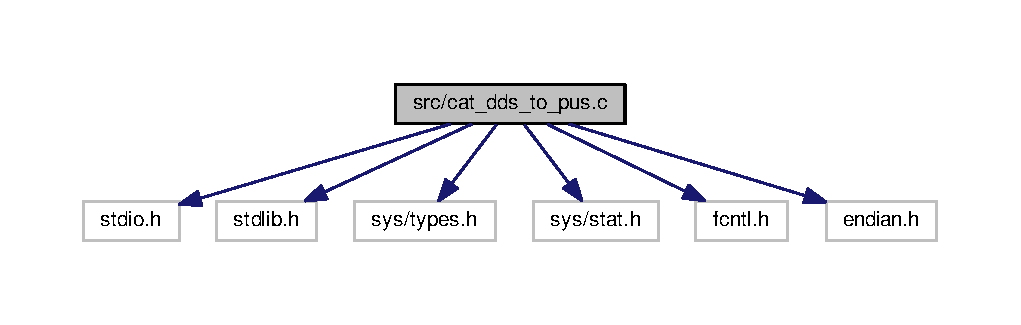
\includegraphics[width=350pt]{cat__dds__to__pus_8c__incl}
\end{center}
\end{figure}


\subsection{Detailed Description}
convert dds file to ccsds pus files from an original program by Jouni Ryno \href{mailto:Jouni.Ryno@fmi.fi}{\tt Jouni.\+Ryno@fmi.\+fi} 





\begin{DoxyAuthor}{Author}
Francesco Lazzarotto \href{mailto:francesco.lazzarotto@inaf.it}{\tt francesco.\+lazzarotto@inaf.\+it} 
\end{DoxyAuthor}
\begin{DoxyCopyright}{Copyright}
2019 G\+PL 2 free software license 
\end{DoxyCopyright}

%--- End generated contents ---

% Index
\backmatter
\newpage
\phantomsection
\clearemptydoublepage
\addcontentsline{toc}{chapter}{Index}
\printindex

\end{document}
